\documentclass[11pt]{article}

% ==== Paquetes ====
\usepackage[utf8]{inputenc}
\usepackage[spanish]{babel}
\usepackage[T1]{fontenc}

\usepackage{amsmath, amssymb, amsfonts, siunitx}
\usepackage{graphicx}
\usepackage{caption}
\usepackage{subcaption}
\usepackage{tikz}
\usepackage{geometry}
\usepackage{float}

\usepackage{hyperref}
\usepackage{minted}
\usepackage{mdframed}
\usepackage{pdfpages}

\usemintedstyle{perldoc}
\geometry{margin=2.5cm}

% ==== Datos de la tarea ====
\title{IEE3584 - Comunicaciones inalámbricas \\
Tarea 11}
\author{Nicolás Seguel}
\date{Noviembre 2025}

\begin{document}

\maketitle

\section*{Problema 28}
\subsection*{(a) Generación de secuencias de desvanecimiento}

Se generaron $N_r = 4$ secuencias de desvanecimiento Rayleigh utilizando la rutina \texttt{fading\_rayleigh\_fd()} del Problema 8, con los mismos parámetros:
\[
v = \SI{60}{km/h}, \quad f_c = \SI{1.8}{GHz}, \quad T_s = \SI{100}{\micro s}, \quad T_d = \SI{0.5}{s}.
\]
Cada secuencia usa una semilla distinta: $[10,\,20,\,30,\,40]$, y se normaliza para que $\mathrm{E}[|h|^2] = 1$, lo que implica una razón señal a ruido media $\bar{\gamma}=1$.

En la Figura~\ref{fig:envelopes} se muestran las envolventes instantáneas $|h_r(t)|$ de las cuatro ramas receptoras, superpuestas. Se verifica que el valor RMS de cada secuencia es cercano a $1$ (0 dB).

\begin{figure}[H]
    \centering
    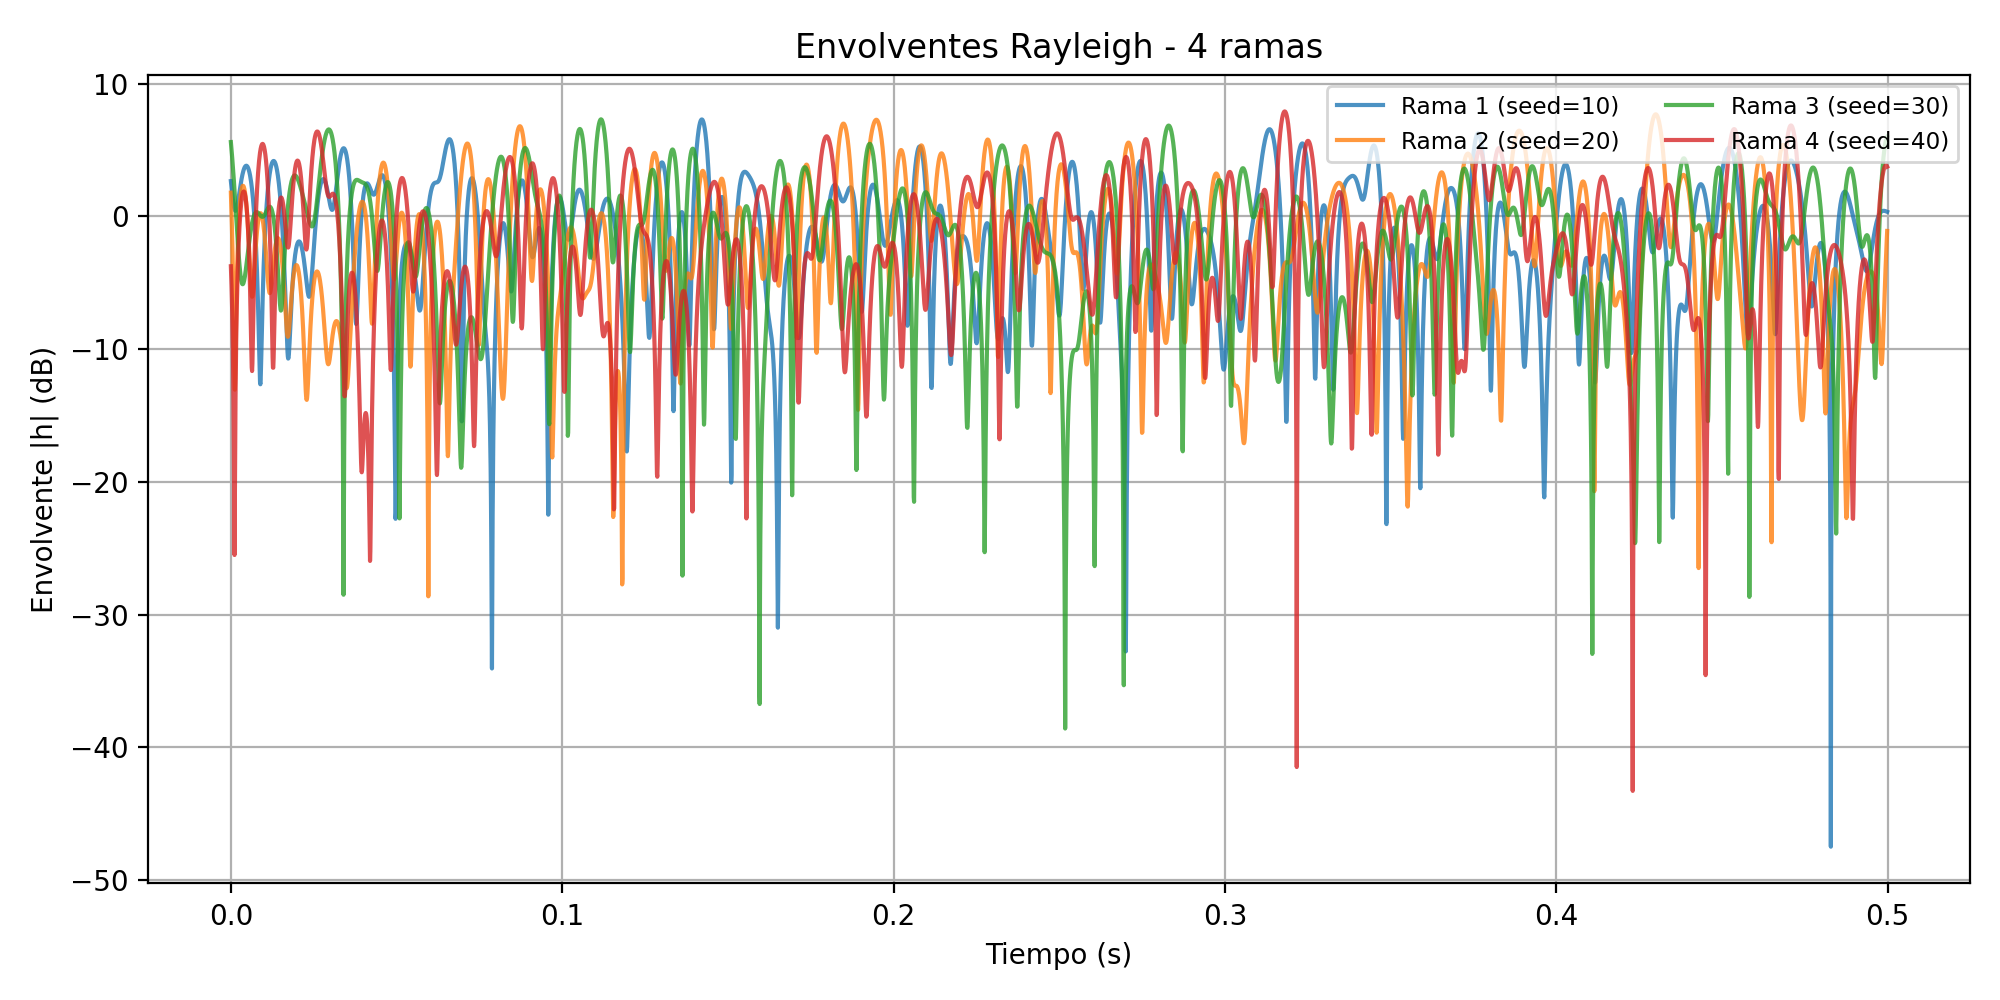
\includegraphics[width=0.9\textwidth]{figs/problema28_envelopes.png}
    \caption{Envolventes Rayleigh $|h_r(t)|$ de las $N_r=4$ ramas.}
    \label{fig:envelopes}
\end{figure}

\subsection*{(b) Combinación MRC y ganancia de arreglo}

Para cada instante discreto $n$, se calcularon los pesos MRC instantáneos:
\[
\hat{u}_r^*(n) = \frac{h_r^*(n)}{\sqrt{\sum_{k=1}^{N_r} |h_k(n)|^2}},
\]
de modo que el vector de pesos maximiza la SNR de salida.  

\begin{figure}
    \centering
    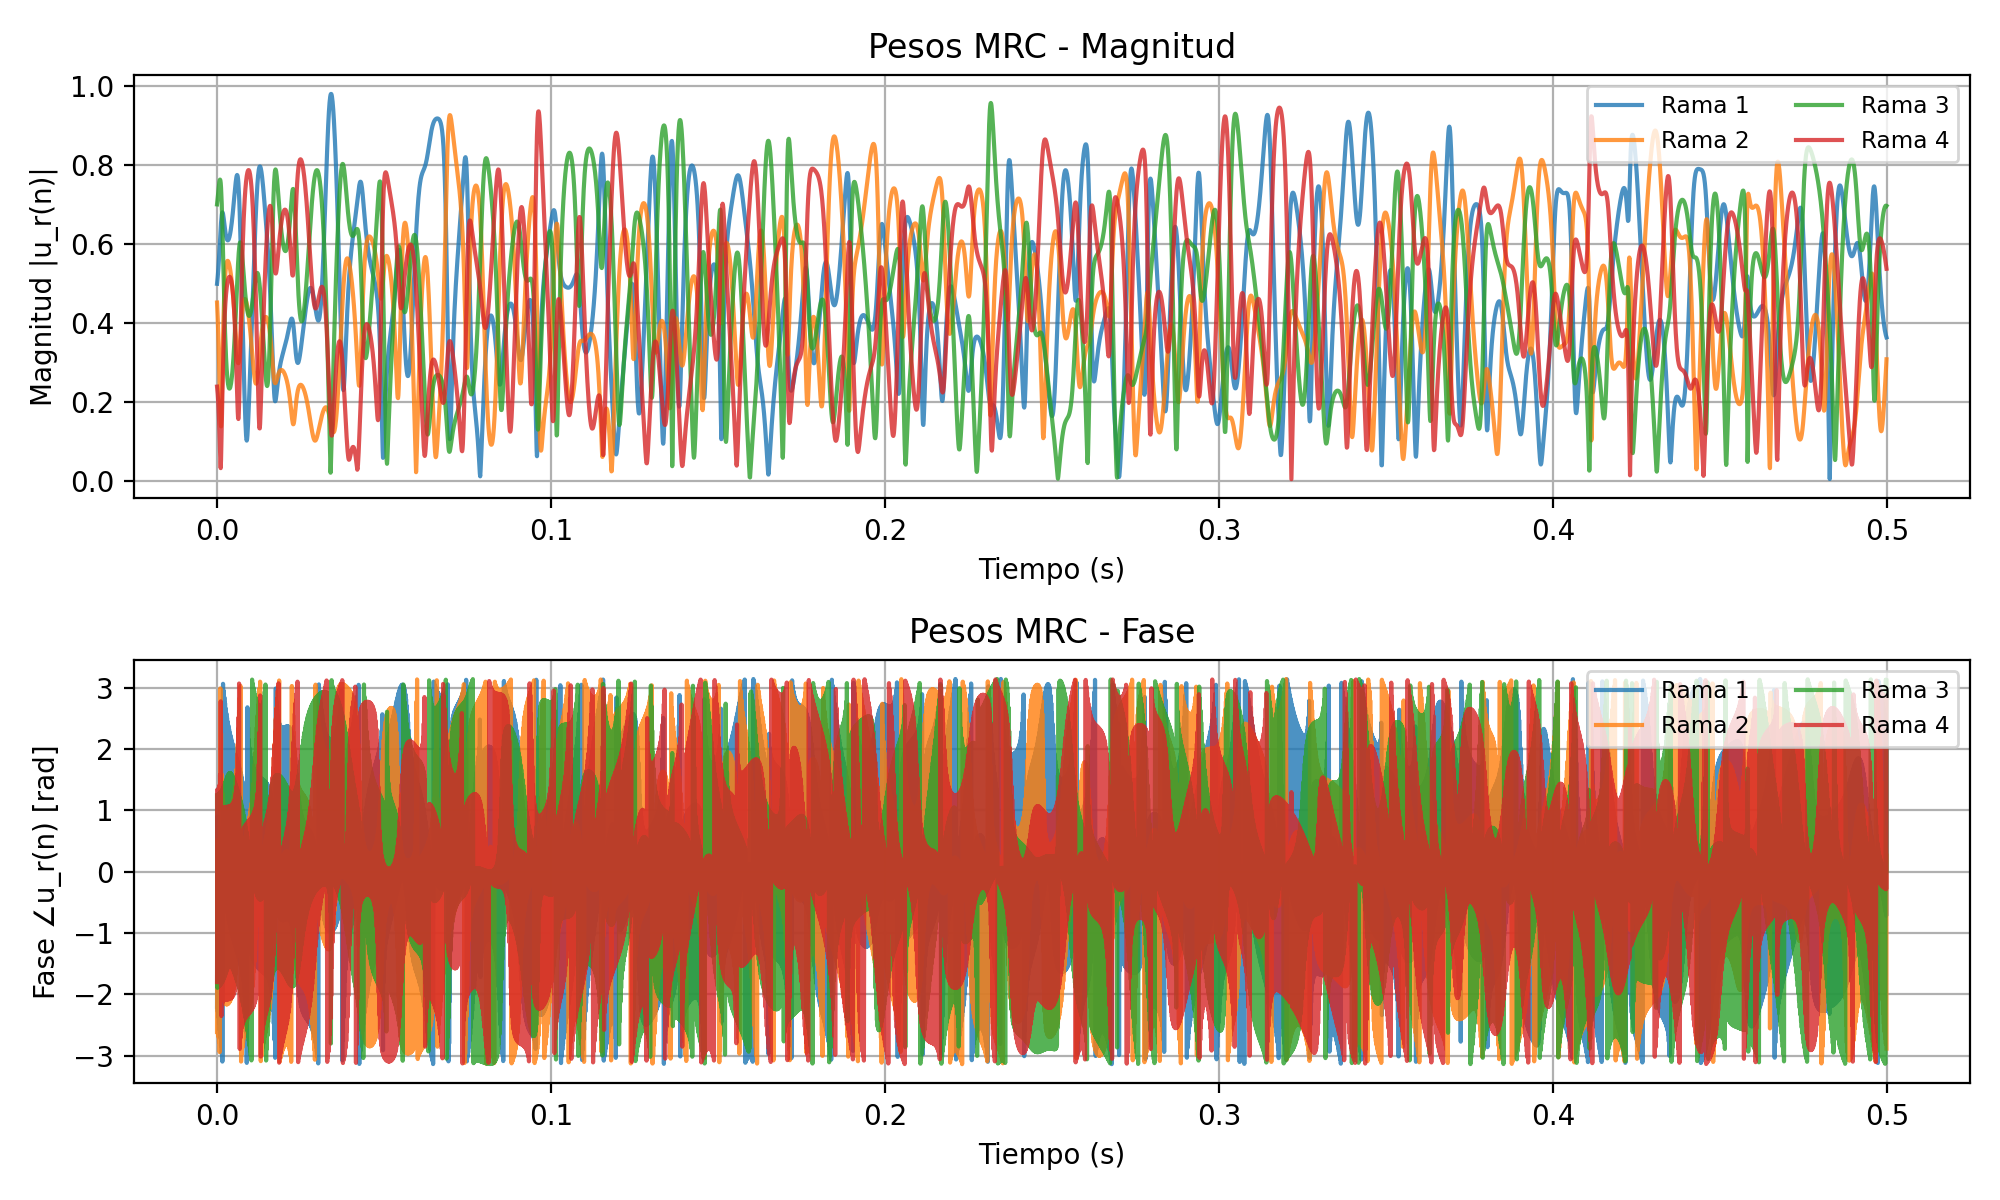
\includegraphics[width=0.9\textwidth]{figs/problema28_mrc_weights.png}
    \caption{Pesos MRC $\hat{u}_r^*(n)$ para las $N_r=4$ ramas.}
    \label{fig:mrc_weights}
\end{figure}

La SNR instantánea de cada rama y de la salida se obtuvo como:
\[
\gamma_r(n) = \bar{\gamma} |h_r(n)|^2, 
\qquad
\Gamma(n) = \bar{\gamma} \sum_{r=1}^{N_r} |h_r(n)|^2.
\]

La Figura~\ref{fig:snr_ramas} muestra las SNR por rama, mientras que la Figura~\ref{fig:snr_out} presenta la SNR de salida del combinador.

\begin{figure}[H]
    \centering
    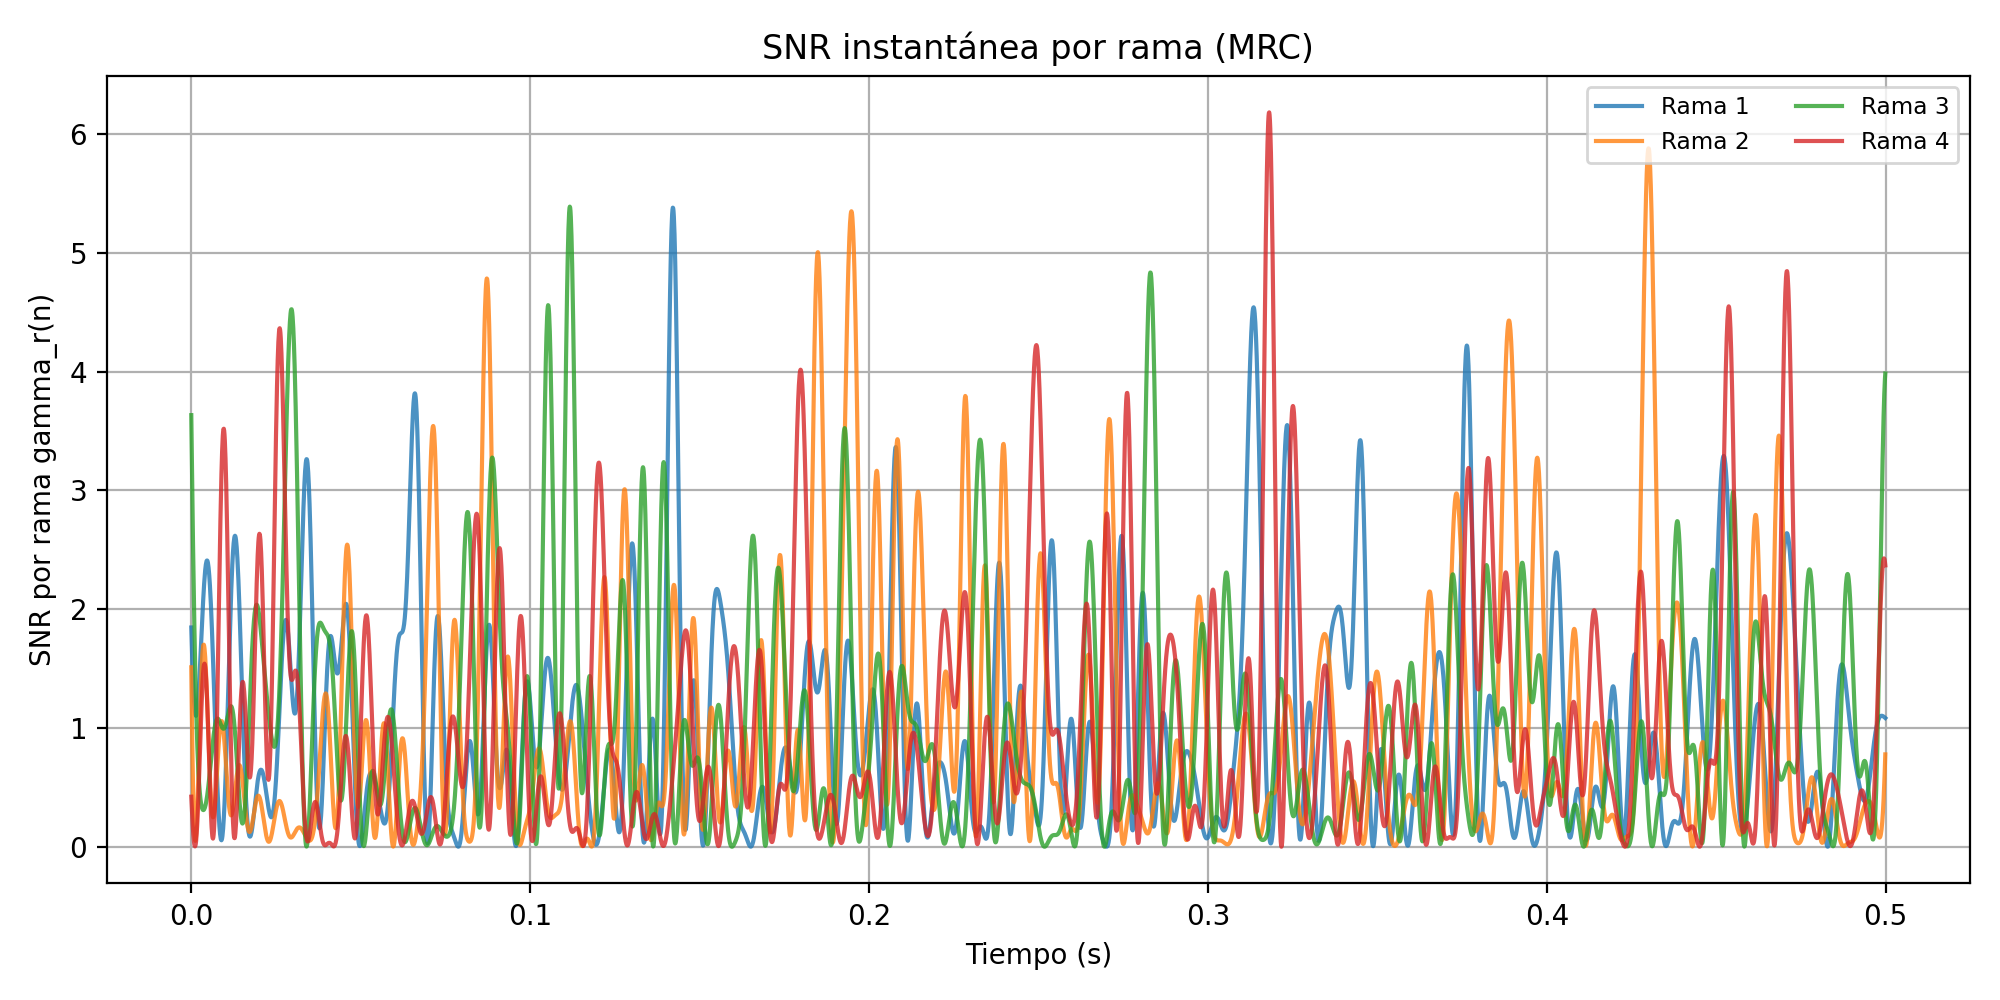
\includegraphics[width=0.9\textwidth]{figs/problema28_gamma_r.png}
    \caption{SNR instantánea por rama $\gamma_r(n)$ en valores lineales.}
    \label{fig:snr_ramas}
\end{figure}

\begin{figure}[H]
    \centering
    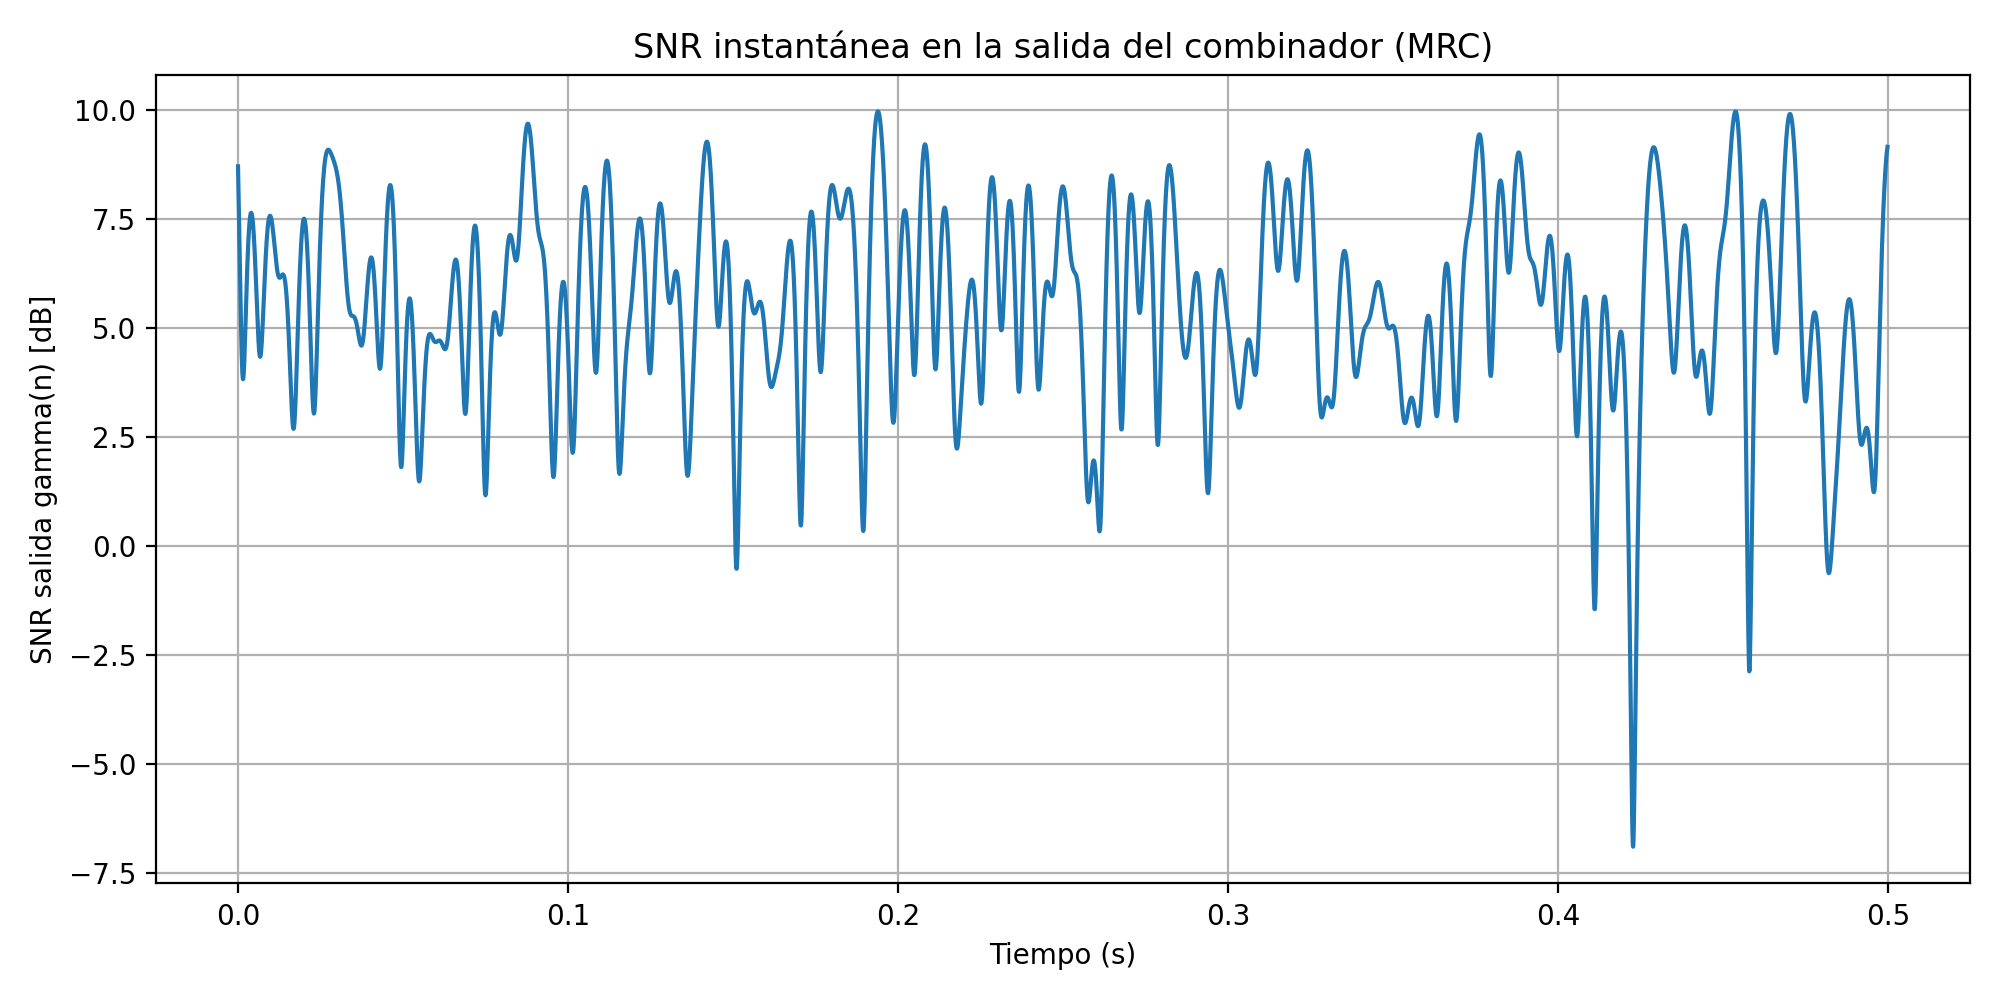
\includegraphics[width=0.9\textwidth]{figs/problema28_Gamma_out.png}
    \caption{SNR instantánea a la salida del combinador MRC, en dB.}
    \label{fig:snr_out}
\end{figure}

El promedio temporal de $\Gamma(n)$ entrega la SNR promedio de salida:
\[
\bar{\Gamma} = \mathrm{E}[\Gamma(n)] \approx 4.01,
\]
de donde la ganancia de arreglo resulta:
\[
G_{\text{arr}} = \frac{\bar{\Gamma}}{\bar{\gamma}} = 4.01 \approx 6.03~\text{dB}.
\]

\subsection*{Comentario}

El resultado coincide con la predicción teórica de una ganancia de $N_r = 4$, es decir,
\[
G_{\text{teo}} = 10\log_{10}(N_r) = 10\log_{10}(4) = 6.02~\text{dB}.
\]
Por tanto, el simulador confirma que el combinador MRC aprovecha completamente la diversidad espacial del arreglo receptor, aumentando linealmente la SNR media con el número de ramas.

\section*{Código fuente}

\begin{mdframed}[backgroundcolor=gray!10,linecolor=black!10]
\inputminted[fontsize=\scriptsize,breaklines]{python}{problema28.py}
\end{mdframed}


\end{document}